%%%%%%%%%%%%%%%%%%%%%%%%%%%%%%%%%%%%%%%%%%%%
% Servo and Stepper Motor Interfacing Presentation
% Author: Joel Manish Pinto and Vishal Rajai
%%%%%%%%%%%%%%%%%%%%%%%%%%%%%%%%%%%%%%%%%%%%

%----------------------------------------------------------------------------------------
%	PACKAGES AND THEMES
%----------------------------------------------------------------------------------------
		
\documentclass[table,10pt,red]{beamer}	% First line -- Define document class as Beamer which is used for creating presentation using Latex
\setbeamercolor{alerted text}{fg=blue} 	% Sets color of highlighted text during presentation.  
 

% The Beamer class comes with a number of default slide themes
% which change the colors and layouts of slides. Below this is a list
% of all the themes, uncomment each in turn to see what they look like.

\usetheme{default}
%\usetheme{AnnArbor}
%\usetheme{Antibes}
%\usetheme{Bergen}
%\usetheme{Berkeley}
%\usetheme{Berlin}		%used theme in present documents.
%\usetheme{Boadilla}
%\usetheme{CambridgeUS}
%\usetheme{Copenhagen}
%\usetheme{Darmstadt}
%\usetheme{Dresden}
%\usetheme{Frankfurt}
%\usetheme{Goettingen}
%\usetheme{Hannover}
%\usetheme{Ilmenau}
%\usetheme{JuanLesPins}
%\usetheme{Luebeck}
%\usetheme{Madrid}
%\usetheme{Malmoe}
%\usetheme{Marburg}
%\usetheme{Montpellier}
%\usetheme{PaloAlto}
%\usetheme{Pittsburgh}
%\usetheme{Rochester}
%\usetheme{Singapore}
%\usetheme{Szeged}
%\usetheme{Warsaw}

% As well as themes, the Beamer class has a number of color themes
% for any slide theme. Uncomment each of these in turn to see how it
% changes the colors of your current slide theme.

%\usecolortheme{albatross}
%\usecolortheme{beaver}
%\usecolortheme{beetle}
%\usecolortheme{crane}
%\usecolortheme{dolphin}
%\usecolortheme{dove}
%\usecolortheme{fly}
%\usecolortheme{lily}
%\usecolortheme{orchid}
%\usecolortheme{rose}
%\usecolortheme{seagull}
%\usecolortheme{seahorse}
%\usecolortheme{whale}
%\usecolortheme{wolverine}

%\setbeamertemplate{footline} % To remove the footer line in all slides uncomment this line
%\setbeamertemplate{footline}[page number] % To replace the footer line in all slides with a simple slide count uncomment this line

%\setbeamertemplate{navigation symbols}{} % To remove the navigation symbols from the bottom of all slides uncomment this line
%}

%------------------------------------------------------------------------------------------
%	\usepackage is required for including various features like images, table, references etc.
%	Packages must be installed before using. These can be istalled through package manager. 
%   Various packages have dependencies and for using such packages all dependent packages must be used. 
%-----------------------------------------------------------------------------------------
\usepackage{beamerthemeshadow} % theme shadow for visual 
\usepackage{beamerthemesplit} % Creates minipage (for showing multiple images and text) on same page  
\usepackage{graphicx} % Allows including images
\usepackage{booktabs} % Allows the use of \toprule, \midrule and \bottomrule in tables
\usepackage{xcolor}
\usepackage{booktabs,array}
\usepackage{listings}
\usepackage{hyperref}	% Required for including hyperlink in document
\usepackage{verbatim,moreverb} % Required for including code snippet.
\usepackage{colortbl}
\usepackage{multirow}	% Required for creating multiple row tables
\usepackage{tikz}		% Required for drawing shapes such as circles, arrowed line, etc. 
\usepackage{gensymb}
\usetikzlibrary{arrows}

% logo
\logo{
\includegraphics[height=1cm]{iitblogo.pdf}} % includes logo at bottom of all slides 

%----------------------------------------------------------------------------------------
%	TITLE PAGE
%----------------------------------------------------------------------------------------
% sf family, bold font
\sffamily \bfseries
% content inside [] appears at bottom of all page. content inside {} appears on first page as title. double backslash means line change 
\title
[
	Servo and Stepper Motor Interfacing	% bottom of all page
	\hspace{2cm}
	\insertframenumber/\inserttotalframenumber
]
{
	Servo and Stepper Motor Interfacing
}

\author
[
	Joel Pinto and Vishal Rajai
]
% author name on title slide
{
	Joel Manish Pinto and Vishal H. Rajai \\
	Under Bhavin Upadhyay \\
	eYantra Summer Internship - 2014\\
	Indian Institute of Technology-Bombay \\
}
\date
{
	IIT Bombay \\ {\today}
}

\begin{document}

\begin{frame}
	\titlepage
\end{frame}

\begin{frame}
	\frametitle{Objective}
	\begin{itemize}
		\item Study of stepper and servo motors
		\item Interfacing with ATmega2560 and ARM based Firebird V robot
		\item Study working characteristics of steppers
		\item Write API for precision and speed control of a servo
		\item Write API for speed control of a stepper
		\item Investigate frequency range supported by servo
		\item Control 4-DOF robotic arm and write API
	\end{itemize}
\end{frame}

%\begin{frame}
%	\frametitle{Scope}
%	\begin{itemize}
%		\item <+-> 
%		\item <+-> 
%		\item <+-> 
%	\end{itemize}
%\end{frame}

\begin{frame}
	\frametitle{Completion}
	\begin{columns}[t]
		\column{.8\textwidth} % Left column and width
		\textbf{Tasks}
		\begin{itemize}
			\item Study of stepper and servo motors
			\item Interfacing with Firebird V robot
			\item Study working characteristics of steppers
			\item Write API for precision and speed control of a servo
			\item Write API for speed control of a stepper
			\item Investigate frequency range supported by servo
			\item Control 4-DOF robotic arm and write API
		\end{itemize}
		\column{.1\textwidth} % Right column and width
		\textbf{Status} \vspace{3.5pt}
		Done \vspace{3.5pt}
		Done \vspace{3.5pt}
		Done \vspace{3.5pt}
		Done \vspace{3.5pt}
		Done \vspace{3.5pt}
		Done \vspace{3.5pt}
		Pending
	\end{columns}
\end{frame}

\begin{frame}
	\frametitle{Results and Discussion}
	\framesubtitle{Stepper Characteristics}
	\begin{itemize}
		\item Stepper's voltage vs. current graphs were analysed for different step modes.
		\begin{figure}
			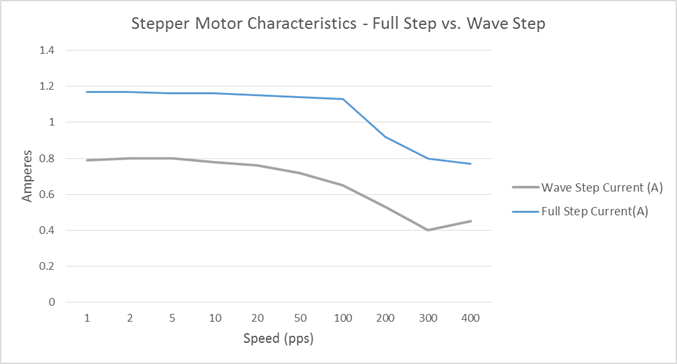
\includegraphics[width=0.8\textwidth]{comparison}
			\caption{Comparison of currents in Full vs Half stepping modes}
		\end{figure}
	\end{itemize}
\end{frame}

\begin{frame}
	\frametitle{Results and Discussion}
	\framesubtitle{Stepper Characteristics (contd.)}
	\begin{itemize}
		\item Stepper's torque at different speeds could not be measured because of the lack of reliable method and equipment to measure the static as well as dynamic torque simultaneously.
	\end{itemize}
	\begin{figure}
		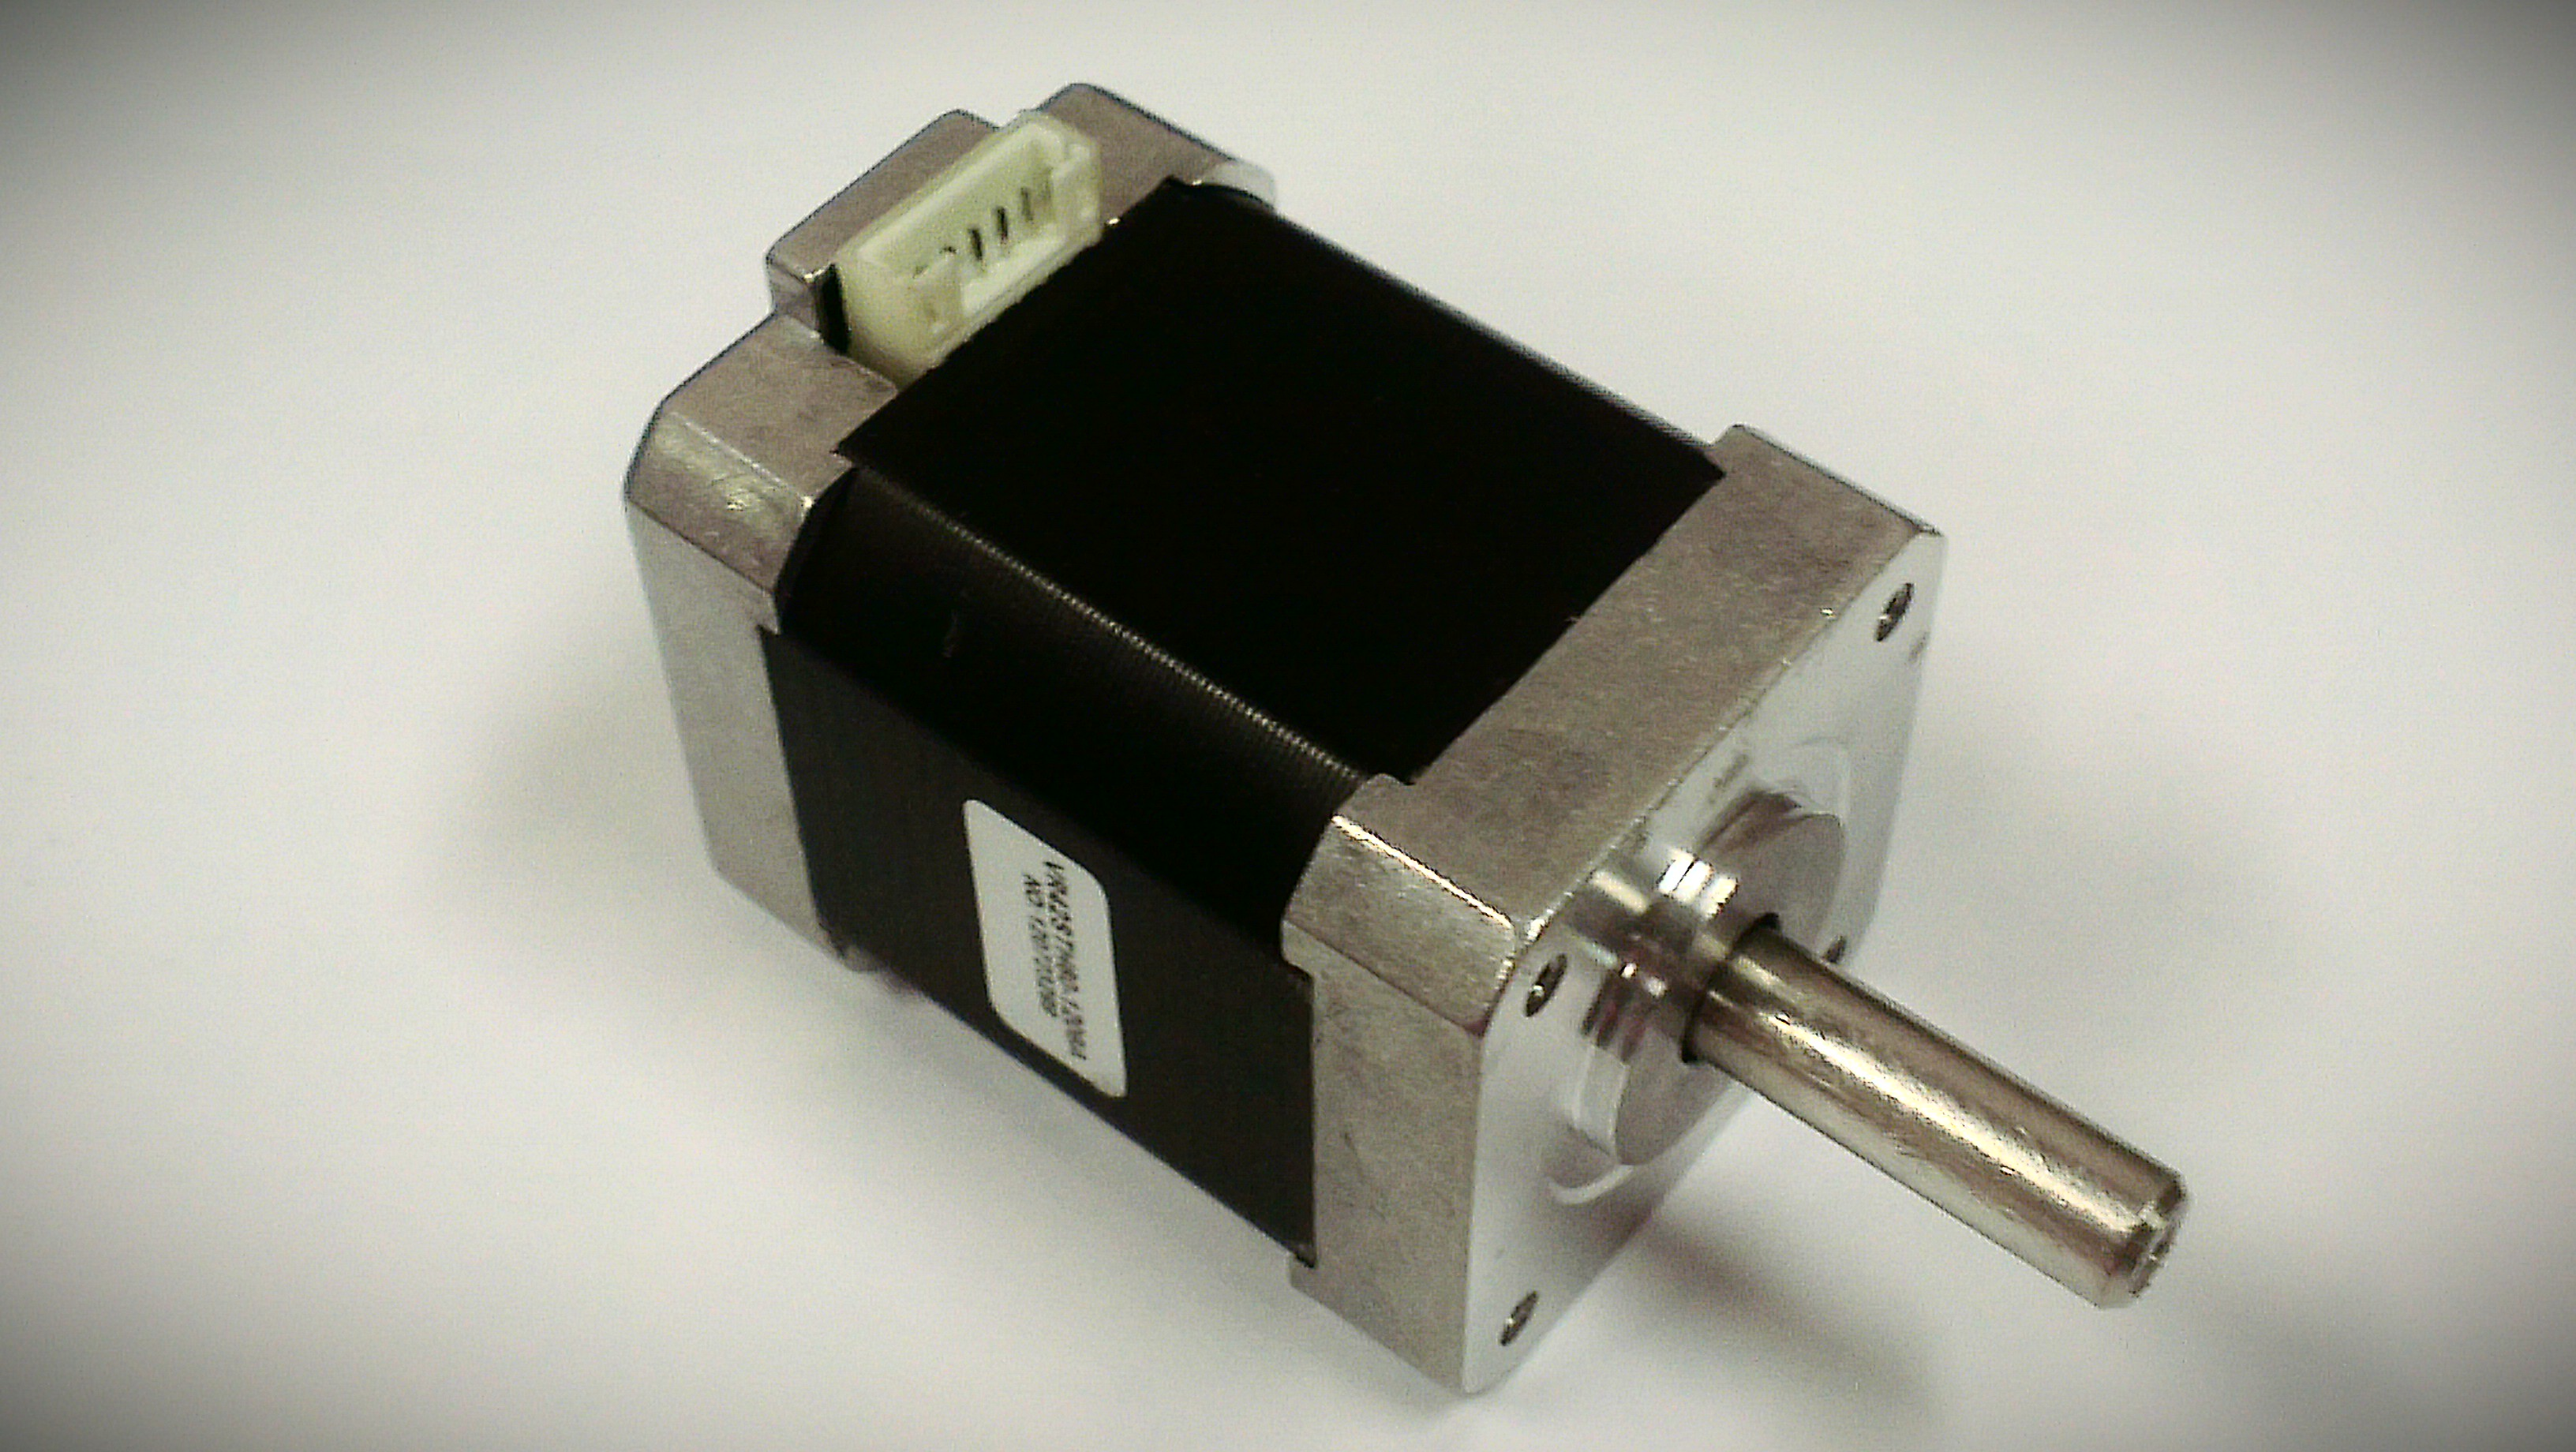
\includegraphics[width=0.7\textwidth]{IMAG0758_1}
	\end{figure}
\end{frame}

\begin{frame}
	\frametitle{Results and Discussion}
	\framesubtitle{Servo Precision and Speed Control API}
	\begin{itemize}
		\item Implemented with interrupts
		\item A 20 ms time period divided into 8 slots of 2.5 ms each
		\item Each used to control the on time of 3 servos with 3 channels of Timer1
		\item Speed is varied by linearly increasing/decreasing servo angle in calculated time
		\begin{figure}
			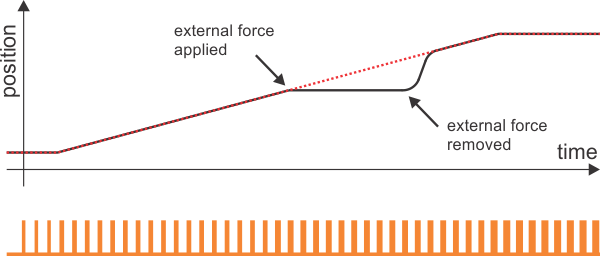
\includegraphics[width=0.6\textwidth]{ramp}
			\caption{Speed control through position ramp}
		\end{figure}
	\end{itemize}
\end{frame}

\begin{frame}
	\frametitle{Results and Discussion}
	\framesubtitle{Stepper Speed Control API}
	\begin{itemize}
		\item Implemented using timer and compare match interrupt
		\item A continuously running timer is used.
		\item Time period before next step is calculated and compare match is scheduled after that time
		\item Speed is varied by varying the step time delay
	\end{itemize}
\end{frame}

\begin{frame}
	\frametitle{Results and Discussion}
	\framesubtitle{Servo characteristics}
	\begin{itemize}
		\item Servo operating frequency $\Rightarrow$ 20 - 300 Hz
		\item Much more tolerant than rated range of 40 - 60 Hz
		\item Torque and speed output fairly constant throughout range
		\item Lower frequencies (5 - 15 Hz) gives low torque and jerky motion
		\item Servo starts heating up at higher frequencies ($>$ 300 Hz)
	\end{itemize}
\end{frame}

\begin{frame}
	\frametitle{Features and bugs}
	\framesubtitle{Servo Precision and Speed Control API}
	\textbf{Features}
	\begin{itemize}
		\item Simultaneous control of upto 24 servos
		\item Servo can be connected to any GPIO pin
		\item $1\degree$ precision for each servo
		\item Independent Speed control
		\item Ability to simultaneously rotate multiple servos
		\item Non-blocking calls - implemented in interrupts
	\end{itemize}
	\textbf{Bugs and Limitations}
	\begin{itemize}
		\item Servo tends to deviate to extreme end when changing targets near $0\degree$
		\item Servo sometimes takes a fast start when told to move at a certain speed
	\end{itemize}
\end{frame}

\begin{frame}
	\frametitle{Features and bugs}
	\framesubtitle{Stepper Speed Control API}
	\textbf{Features}
	\begin{itemize}
		\item Stepper can be connected to any GPIO pins even from different ports
		\item Upto 3 steppers can be controlled simultaneously
		\item Steppers can be commanded to rotate in single steps or to rotate specified number of steps at a specified speed
		\item Speed can be varied in motion to create speed ramps
		\item Non-blocking calls - implemented in interrupts
	\end{itemize}
	\textbf{Bugs and Limitations}
	\begin{itemize}
		\item Only 3 steppers can be controlled with a single timer.
		\item Speed ramps aren't implemented in interrupts although it is possible
	\end{itemize}
\end{frame}

\begin{frame}
	\frametitle{Future Work}
	\begin{itemize}
		\item Stepper API can be improved to implement speed ramp in interrupts
		\item Servo API can be used for robotic arms and humanoid robots requiring simultaneous control of multiple servos
		\item Resolving bugs in Servo API
	\end{itemize}
\end{frame}

\begin{frame}
	\frametitle{B.E. Project Idea}
	\framesubtitle{Joel}
	\textbf{Environment mapping and shortest path planning}
	\begin{itemize}
		\item A robot examining its surroundings and building a map in memory.
		\item Then on further navigations to a certain destination, use the shortest path to travel to it
		\item Can be applied in situations or places where human exploration is limited or dangerous.
	\end{itemize}
	\begin{figure}
		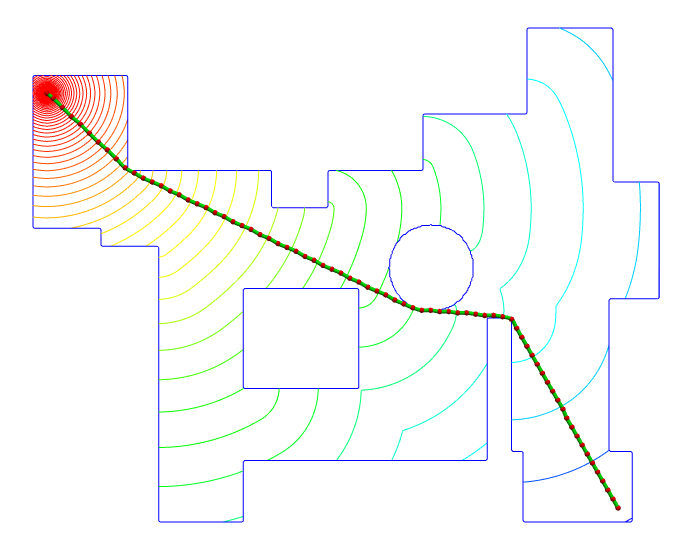
\includegraphics[width=0.5\linewidth]{shortest}
	\end{figure}
\end{frame}

\begin{frame}
	\frametitle{B.E. Project Idea}
	\framesubtitle{Vishal}
	\textbf{Control of Wheelchair using Eye Movements}
	\begin{itemize}
		\item A camera captures images.
		\item Sends these to a computer for processing
		\item Depending on pics of various eye, head movements, sends commands to controller for doing certain task
	\end{itemize}
\end{frame}

\begin{frame}
	\frametitle{B.E. Project Idea}
	\framesubtitle{Vishal}
	\textbf{Control of Wheelchair using BCI}
	\begin{itemize}
		\item An electrode captures neural signals
		\item Sends these to a computer for processing
		\item Depending on peaks in signals due to various movements, sends commands to controller for doing certain task
	\end{itemize}
\end{frame}

\begin{frame}
\begin{center}
\textbf{\LARGE Thank You!}
\end{center}

\end{frame}

\end{document} 